\documentclass[aspectratio=169]{beamer}
\usetheme{Boadilla}
\setbeamertemplate{navigation symbols}{}
\usepackage{graphicx} % Required for inserting images
\graphicspath{{./figures}}
\usepackage[autostyle=true]{csquotes}
\usepackage[T2A]{fontenc}
\usepackage[english, russian]{babel}

\title{Interactive Speaker Recognition}
\subtitle{Применение обучения с подкреплением для решения задачи распознавания
          диктора}
\author[В.С.~Головин]{Вячеслав Головин \texorpdfstring{\newline}{, }
    {\small Евгений Шуранов (руководитель)}}
\institute[ВШЭ]{Huawei CBG AI и ФКН ВШЭ СПб}
\date{16.05.2023}

\newcommand{\guesser}{\texttt{Guesser}}
\newcommand{\enquirer}{\texttt{Enquirer}}
\newcommand{\imgscale}{0.8}

\begin{document}

\frame{\titlepage}

\begin{frame}{}
    \textbf{Задача:} повышение точности систем верификации / идентификации
    диктора. Такая система может, например, быть использована для подтверждение
    личности на мобильных устройствах.\vspace{1em}

    \textbf{Требования к системе:}
    \begin{itemize}
        \item короткие запросы (не раздражаем пользователя),
        \item разнообразные запросы (не боимся спуфинга),
        \item высокая точность (без комментариев).
    \end{itemize}\vspace{1em}

    \textbf{Предлагаемое решение:} использование RL-агента для выбора
    запрашиваемых слов.\vspace{1em}

    \textbf{Новизна дипломной работы:}
    \begin{itemize}
        \item переход от идентификации к верификации,
        \item более гибкая система для выбора слов.
    \end{itemize}
\end{frame}

\begin{frame}{Interactive Speaker Recognition}
    Метод был предложен в статье \textit{A Machine of Few Words --- Interactive
    Speaker Recognition with Reinforcement Learning}, Mathieu Seurin et al.,
    INTERSPEECH 2020, arXiv:2008.03127v1.\vspace{1em}

    \begin{columns}
    
    \column{0.6\textwidth}
    \begin{figure}[bht]
        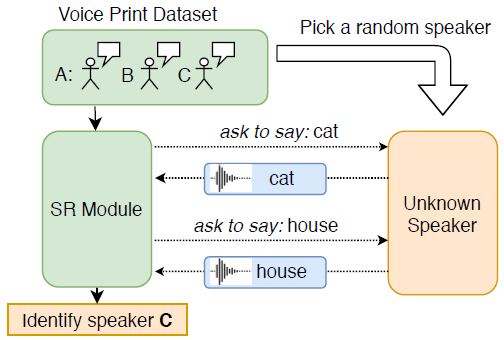
\includegraphics[width=.9\textwidth]{isr_game_large.png}
        % \caption{Общая схема подхода ISR}
    \end{figure}

    \column{0.4\textwidth}
    Важные особенности:
    \begin{enumerate}
        \item Рассматривается только задача идентификации.
        \item Набор слов строго фиксирован.
        \item Разные нейронные сети для двух задач SR Module --- запроса слов
        (\enquirer) и идентификации диктора (\guesser).
    \end{enumerate}
    \end{columns}
\end{frame}

\begin{frame}{Блок Guesser}
\framesubtitle{Архитектура}
    \begin{columns}
    
    \column{0.6\textwidth}
    \begin{figure}[bht]
    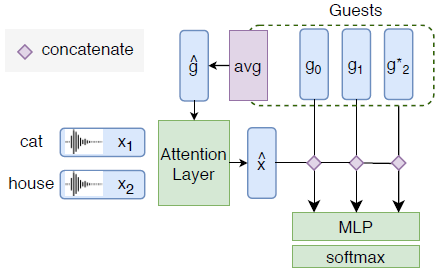
\includegraphics[width=.8\textwidth]{guesser.png}
    % \caption{Архитектура блока Guesser}
    \end{figure}

    \column{0.4\textwidth}
    Входные данные:
    \begin{itemize}
        \item эмбеддинги дикторов\\
            $G = [g_1; g_2; \ldots g_K]$
        \item эмбеддинги слов\\
            $X = [x_1; x_2; \ldots x_T]$
    \end{itemize}
    Выходные данные:
    \begin{itemize}
        \item вероятности
            $\{P(g_i = g^*) \;|\; i=1..K\}$
    \end{itemize}
    \end{columns}

    \begin{block}{Обозначения}
    \begin{tabular}{l l}
        $K$ & количество гостей / дикторов\\
        $T$ & количество запрашиваемых слов
    \end{tabular}
    \end{block}
\end{frame}

\begin{frame}[fragile]{Блок Guesser}
\framesubtitle{Псевдокод 1 итерации обучения}
\begin{lstlisting}[caption={Рассчёт функции потерь \guesser{}}]
speaker_ids = speakers.sample(size=K)
G = voice_prints.get(speaker_ids)
target = randrange(0, K)
word_inds = randrange(0, V, size=T)
X = word_vocab.get(speaker=speaker_ids[target],
                   words=word_inds)
probabilities = guesser.forward(G, X)
loss = cross_entropy(probabilities, target)
\end{lstlisting}
    \begin{block}{Обозначения}
    \begin{tabular}{l l}
        $K$ & количество гостей / дикторов\\
        $T$ & количество запрашиваемых слов\\
        $V$ & размер словаря --- число доступных для запроса слов
    \end{tabular}
    \end{block}
\end{frame}

\begin{frame}{Блок Enquirer}
\framesubtitle{Архитектура}
    \begin{columns}
    
    \column{0.6\textwidth}
    \begin{figure}[bht]
    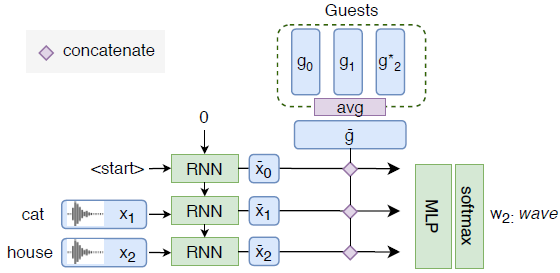
\includegraphics[width=.9\textwidth]{enquirer.png}
    % \caption{Архитектура блока Enquirer}
    \end{figure}

    \column{0.4\textwidth}
    Входные данные:
    \begin{itemize}
        \item среднее эмб. дикторов\\
            $\hat{g} = \frac{1}{K}{\sum_{i=1}^{K}{g_k}}$
        \item эмбеддинги слов\\
            $X = [x_1; x_2; \ldots; x_t]$
    \end{itemize}
    Выходные данные:
    \begin{itemize}
        \item вероятность выбрать каждое из слов
    \end{itemize}

    \end{columns}

    \begin{block}{Обозначения}
    \begin{tabular}{l l}
        $K$ & количество гостей / дикторов\\
        $T$ & количество запрашиваемых слов\\
        $t$ & количество запрошенных слов, $0 \leq t \leq T$
    \end{tabular}
    \end{block}
\end{frame}

\begin{frame}[fragile]{Блок Enquirer}
\framesubtitle{Псевдокод 1 эпизода ISR-игры}
\footnotesize
\begin{lstlisting}[caption={Интерактивная игра для обучения \enquirer{}}]
speaker_ids = speakers.sample(size=K)
G = voice_prints.get(speaker_ids)
target = randrange(0, K)

g_hat = G.mean(dim=0)
x_i = start_tensor
X = []
for i in range(T):
    probs = enquirer.forward(g_hat, x_i)
    if training:
        word_inds = multinomial(probs).sample()
    else:
        probs[previous_actions] = 0.0
        word_ind = argmax(probs)
    x_i = word_vocab.get(speaker=speaker_ids[target],
                         word=word_ind)
    X.append(x_i)

prediction = guesser.predict(G, X)
reward = 1 if prediction == target else 0
\end{lstlisting}
\end{frame}

\begin{frame}{Входные данные}
    Для обучения использовался датасет \textbf{TIMIT}:
    \begin{itemize}
        \item 630 дикторов из США, 8 акцентов;
        \item каждый диктор произносит 10 предложений: 8 уникальных и 2 общих.
    \end{itemize}

    В качестве эмбеддингов использовались \textbf{x-vectors}, полученные с помощью нейронной сети, обученной на аугментированных датасетах для распознавания диктора \textit{Switchboard}, \textit{Mixer 6} и \textit{NIST}.
    \begin{itemize}
        \item Эмбеддинги дикторов $g$ получались с помощью усреднения
        эмбеддингов 8 уникальных предложений.
        \item Эмбеддинги слов $x$ извлекались с помощью 2 общих предложений,
        т.е. сначала вырезались записи одиночных слов, которые затем
        пропускались через нейронную сеть.
    \end{itemize}
\end{frame}

\begin{frame}{Результаты из статьи}
    \framesubtitle{$K = 5$ дикторов и $T = 3$ слова}
    \begin{columns}
        \centering
        \column{.5\textwidth}
        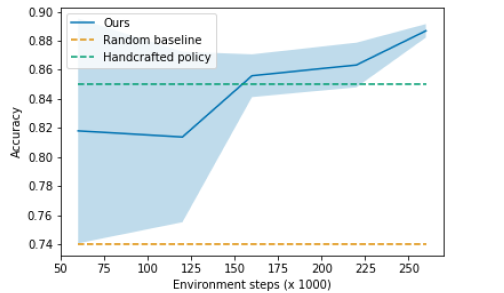
\includegraphics[scale=0.5]{isr_training.png}
        \column{.5\textwidth}
        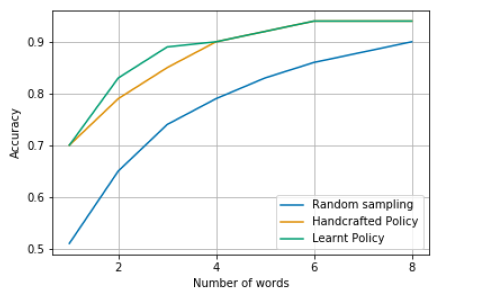
\includegraphics[scale=0.5]{isr_word_sweep.png}
    \end{columns}\vspace*{1em}

    RL-агент при выборе запрашиваемых слов учитывает контекст --- он опережает
    не только случайного агента, но и эвристического, выбирающего из
    подмножества ``лучших'' слов.\vspace*{1em}

    Преимущество RL-агента невелико и проявляется только при небольшом числе
    запрашиваемых слов.
\end{frame}

\begin{frame}{Обучение и тестирование \guesser{}}
    \framesubtitle{$K = 5$ дикторов  и $T = 3$ слова при обучении}
    \begin{columns}
        \centering
        \column{.5\textwidth}
        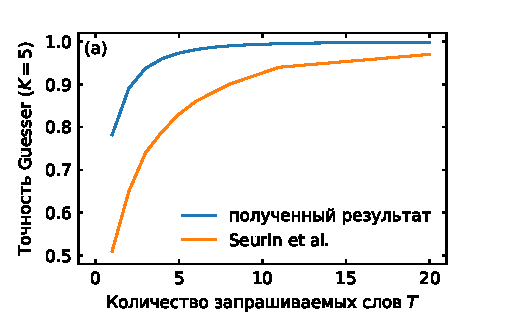
\includegraphics[scale=\imgscale]{../plots/word_sweep.pdf}
        \column{.5\textwidth}
        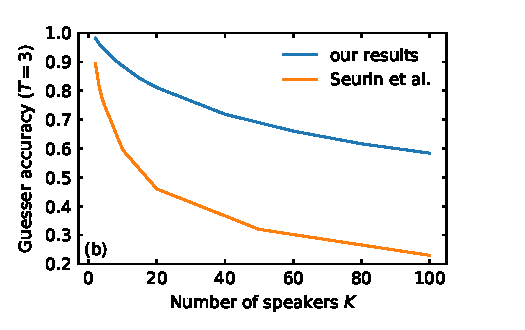
\includegraphics[scale=\imgscale]{../plots/guest_sweep.pdf}
    \end{columns}\vspace*{1em}

    Вероятно, главная причина расхождения результатов --- увеличение размерности
    эмбеддингов (512 вместо 128 в статье). Неизвестно, как и зачем в статье
    производилось понижение размерности.
\end{frame}

\begin{frame}{Обучение и тестирование \enquirer{}}
    \framesubtitle{$K = 5$ дикторов  и $T = 3$ слова при обучении}
    \begin{columns}
        \centering
        \column{.5\textwidth}
        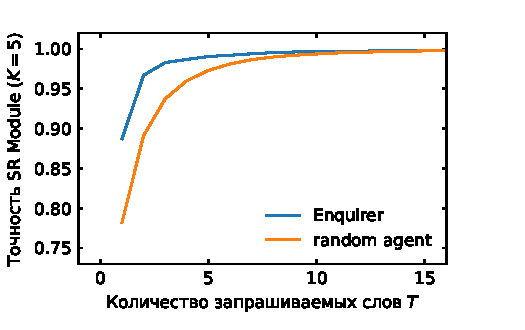
\includegraphics[scale=\imgscale]{../plots/word_sweep_enq.pdf}
        \column{.5\textwidth}
        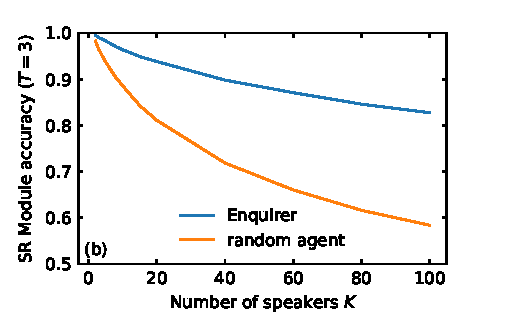
\includegraphics[scale=\imgscale]{../plots/guest_sweep_enq.pdf}
    \end{columns}\vspace*{1em}
    Для обучения использовалась \textbf{PPO}. Выбор слова при обучении и
    тестировании проводился по-разному:
    \begin{itemize}
        \item \texttt{train} --- сэмплирование из распределения,
        \item \texttt{test} --- $\arg \max$ по не использованным ранее словам.
    \end{itemize}
\end{frame}

\begin{frame}{Эвристический агент}
    \framesubtitle{Алгоритм работы}
    \begin{columns}[c]
        \column{.3\textwidth}
        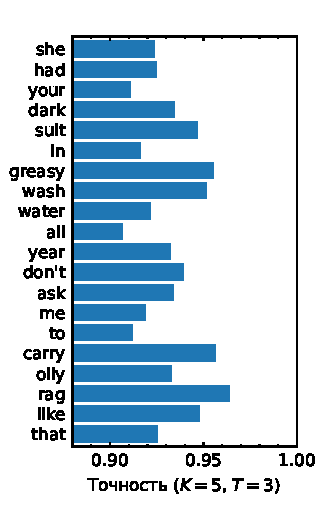
\includegraphics[height=.8\textheight]{../plots/word_scores.pdf}
        \column{.7\textwidth}
        \begin{center}
            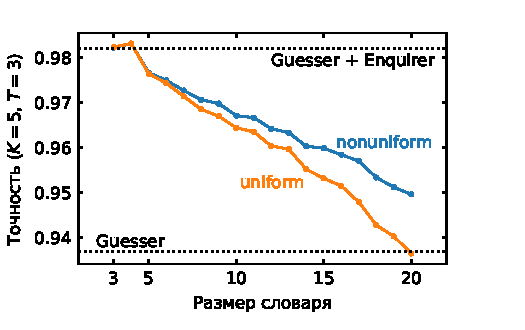
\includegraphics[scale=\imgscale]{../plots/heuristic.pdf}
        \end{center}
        \begin{enumerate}
            \item Рассчитываем точность на валидационной выборке.
            \item Сэмплируем из слов с самой высокой точностью.
        \end{enumerate}
    \end{columns}
\end{frame}

\begin{frame}{Эвристический агент}
    \framesubtitle{Сравнение с \enquirer}
    \begin{columns}
        \centering
        \column{.5\textwidth}
        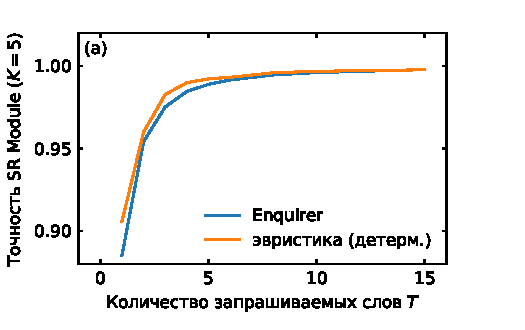
\includegraphics[scale=\imgscale]{../plots/word_sweep_heuristic.pdf}
        \column{.5\textwidth}
        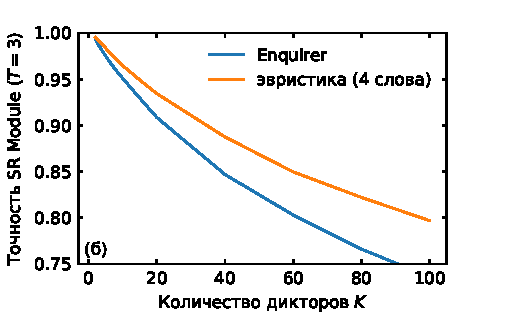
\includegraphics[scale=\imgscale]{../plots/guest_sweep_heuristic.pdf}
    \end{columns}\vspace*{1em}
\end{frame}


\begin{frame}{Верификация}
    \framesubtitle{Как преобразовать \guesser}

    \begin{columns}
        \column{0.6\textwidth}
        \begin{figure}[bht]
        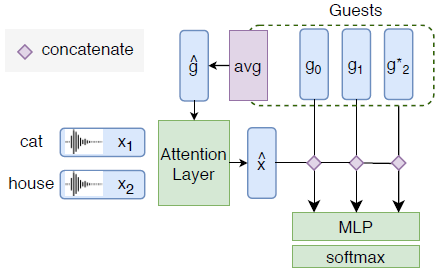
\includegraphics[width=.8\textwidth]{guesser.png}
        \end{figure}

        \column{0.4\textwidth}
        \begin{itemize}
            \item только 1 диктор $\implies$ $\hat{g} = g_0$
            \item \texttt{softmax} $\rightarrow$ \texttt{sigmoid} 
            \item при $T = 3$ точность 0.91\\($\sim$ как в классификации с
                  $K = 7$ гостями)
            \item \texttt{MLP} $\rightarrow$ \texttt{CosineSimilarity} тоже
                  работает, но хуже
        \end{itemize}
    \end{columns}
\end{frame}

\end{document}
